\section{Impact of external linear solver on performance} \label{s:results:performance-external-linear-solver}
Crank--Nicolson scheme requires to solve a linear equation \eqref{eq:crani-nicolson:matrix}. It should be solved as fast as possible to increase to performance of numerical scheme. This section will check if implemented solver is faster than external one used \gls{eigen} library. This verification is made only for serial code. 

Implementation of this problem uses tridiagonal matrix algorithm, also known as the Thomas algorithm, which has a complexity of $\mathcal{O}(n)$. Solution with external library uses $LU$ factorization to solve the problem. This method has complexity of $\mathcal{O}(n^3)$, but knowing that matrix $A$ it is possible to reduce the complexity of problem to $\mathcal{O}(n^2)$ by saving the calculated matrices $LU$.
\begin{figure}[!htbp]
	\centering
	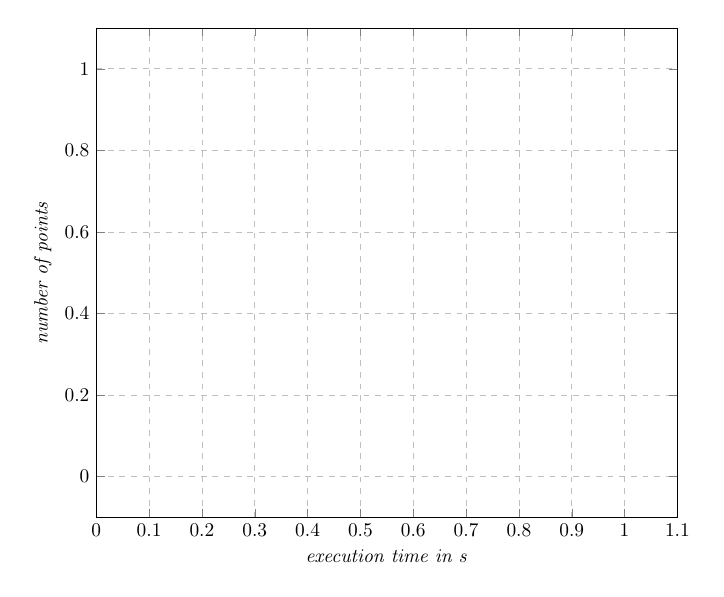
\begin{tikzpicture}[scale=0.7]	 	
	\pgfplotsset{width=\textwidth}
		\begin{axis}[
			xlabel = {\emph{execution time in s}},
			ylabel = {\emph{number of points}},
			%ymin = -1, ymax = 1,
			xmin = 0,% xmax = 13,
			%minor y tick num = 1,
			ymajorgrids=true,
			xmajorgrids=true,
			grid style=dashed,
			legend pos=north west
			]
			\addcustomplot{others/performance/serial-parallel.csv}{cyan}{2}{External library -- \gls{eigen}}
			\addcustomplot{others/performance/serial-parallel.csv}{magenta}{1}{Thomas algorithm}
		\end{axis}
	\end{tikzpicture}
	\caption{Impact of external library linear set solver on Crank-Nicolson schema.}
	\label{fig:imapct:crank-nicolson}
\end{figure}
Tests were performed on \gls{astral} using different grid sizes to show the execution times. The characteristics of used methods are visible in Figure \ref{fig:imapct:crank-nicolson}. The execution times for external library seems to have polynomial dependency, which is expected and connected to complexity of the solver. The results for Thomas algorithm are really good and as expected better than linear solver implemented in \gls{eigen} library. 